\documentclass[12pt,a4paper]{article}

% ─── Page Layout ───────────────────────────────────────────────────────────────
\usepackage[a4paper, margin=0.8in, headheight=14pt]{geometry}

% ─── Fonts (XeLaTeX) ───────────────────────────────────────────────────────────
\usepackage{fontspec}
\usepackage{unicode-math}
\setmainfont{TeX Gyre Pagella}
\setmonofont[Scale=0.88]{TeX Gyre Cursor}
\setmathfont{Latin Modern Math}

% ─── Packages ──────────────────────────────────────────────────────────────────
\usepackage{xcolor}
\usepackage{colortbl}
\usepackage{titlesec}
\usepackage{enumitem}
\usepackage{tabularx}
\usepackage{booktabs}
\usepackage{array}
\usepackage{amsmath}
\usepackage{tikz}
\usetikzlibrary{shapes.geometric, arrows.meta, positioning, calc, fit, decorations.pathreplacing, patterns}
\usepackage{tcolorbox}
\tcbuselibrary{skins, breakable}
\usepackage{hyperref}
\usepackage{fancyhdr}
\usepackage{graphicx}
\usepackage{microtype}
\hyphenpenalty=10000
\exhyphenpenalty=10000
\sloppy
\usepackage{caption}
\usepackage{setspace}
\usepackage{multirow}
\usepackage{tocloft}

% ─── Q&A helper ────────────────────────────────────────────────────────────────
\newcommand{\Q}[1]{\textbf{#1}\par\noindent\ignorespaces}

% ─── Colour Palette ────────────────────────────────────────────────────────────
\definecolor{myred}{RGB}{196,30,58}
\definecolor{mydark}{RGB}{30,30,50}
\definecolor{mygreen}{RGB}{14,120,80}
\definecolor{myteal}{RGB}{0,130,140}
\definecolor{myamber}{RGB}{180,100,0}
\definecolor{mypurple}{RGB}{100,30,160}
\definecolor{mygray}{RGB}{246,247,249}
\definecolor{mgframe}{RGB}{180,185,200}
\definecolor{watermark}{RGB}{145,150,170}
\definecolor{hdrred}{RGB}{250,232,235}
\definecolor{hdrgreen}{RGB}{220,244,233}
\definecolor{hdrteal}{RGB}{220,242,244}
\definecolor{hdramber}{RGB}{253,242,215}
\definecolor{hdrpurple}{RGB}{238,228,255}
\definecolor{hdrgray}{RGB}{238,240,245}
\definecolor{rowalt}{RGB}{250,251,253}

% ─── Section Formatting ────────────────────────────────────────────────────────
\titleformat{\section}
  {\large\bfseries\color{myred}}{\thesection.}{0.5em}{}
  [\vspace{1pt}{\color{myred}\rule{\linewidth}{0.8pt}}]
\titleformat{\subsection}
  {\normalsize\bfseries\color{myteal}}{\thesubsection}{0.5em}{}
\titlespacing*{\section}{0pt}{18pt}{7pt}
\titlespacing*{\subsection}{0pt}{11pt}{4pt}

% ─── Paragraph ─────────────────────────────────────────────────────────────────
\setlength{\parindent}{0pt}
\setlength{\parskip}{4pt}

% ─── TOC Styling ───────────────────────────────────────────────────────────────
\renewcommand{\cfttoctitlefont}{\large\bfseries\color{myred}}
\renewcommand{\cftaftertoctitle}{\par\noindent{\color{myred}\rule{\linewidth}{0.8pt}}}
\setlength{\cftbeforetoctitleskip}{0pt}
\setlength{\cftaftertoctitleskip}{6pt}
\renewcommand{\cftsecfont}{\normalsize\bfseries\color{mydark}}
\renewcommand{\cftsecpagefont}{\normalsize\bfseries\color{mydark}}
\renewcommand{\cftsecleader}{\cftdotfill{\cftdotsep}}
\setlength{\cftbeforesecskip}{7pt}
\renewcommand{\cftsubsecfont}{\small\color{mydark}}
\renewcommand{\cftsubsecpagefont}{\small\color{mydark}}
\setlength{\cftbeforesubsecskip}{3pt}
\setlength{\cftsubsecindent}{1.4em}

% ─── Table helpers ─────────────────────────────────────────────────────────────
\renewcommand{\arraystretch}{1.45}
\setlength{\tabcolsep}{6pt}
\arrayrulecolor{mydark}
\newcolumntype{B}[1]{>{\small\bfseries\raggedright\arraybackslash}m{#1}}
\newcolumntype{Y}{>{\small\raggedright\arraybackslash}X}
\renewcommand{\tabularxcolumn}[1]{m{#1}}

% ─── Header / Footer ───────────────────────────────────────────────────────────
\pagestyle{fancy}
\fancyhf{}
\fancyhead[L]{\small\color{myred}\textbf{EC401}\;\color{mydark}--- Analog Communication}
\fancyhead[R]{\small\color{myteal}\textbf{Module 3 Notes}}
\fancyfoot[C]{\small\color{mydark}\thepage}
\fancyfoot[R]{\small\color{watermark}\textit{\copyright\ Biraj}}
\renewcommand{\headrulewidth}{0.5pt}
\renewcommand{\footrulewidth}{0.3pt}

% ─── Hyperref ──────────────────────────────────────────────────────────────────
\hypersetup{
  colorlinks=true, linkcolor=myteal, urlcolor=myteal,
  pdfauthor={Biraj Sarkar (CGEC)},
  pdftitle={EC401 --- Module 3 Notes: Angle Modulation, Generation and Demodulation}
}

% ─── tcolorbox styles ──────────────────────────────────────────────────────────
\tcbset{
  tikzbox/.style={
    colback=mygray, colframe=mgframe, boxrule=0.6pt, arc=4pt,
    left=8pt, right=8pt, top=6pt, bottom=6pt,
    colbacktitle=mgframe, coltitle=mydark, fonttitle=\small\bfseries
  },
  defbox/.style={
    colback=hdrgreen, colframe=mygreen, boxrule=0.8pt, arc=4pt,
    left=9pt, right=9pt, top=6pt, bottom=6pt,
    colbacktitle=mygreen, coltitle=white, fonttitle=\small\bfseries
  },
  formulabox/.style={
    colback=hdrteal, colframe=myteal, boxrule=0.8pt, arc=4pt,
    left=9pt, right=9pt, top=7pt, bottom=7pt,
    colbacktitle=myteal, coltitle=white, fonttitle=\small\bfseries
  },
  examplebox/.style={
    colback=hdramber, colframe=myamber, boxrule=0.8pt, arc=4pt,
    left=9pt, right=9pt, top=6pt, bottom=6pt,
    colbacktitle=myamber, coltitle=white, fonttitle=\small\bfseries
  },
  masonbox/.style={
    colback=hdrpurple, colframe=mypurple, boxrule=0.8pt, arc=4pt,
    left=9pt, right=9pt, top=6pt, bottom=6pt,
    colbacktitle=mypurple, coltitle=white, fonttitle=\small\bfseries
  },
  exambox/.style={
    colback=hdrpurple, colframe=mypurple, boxrule=1pt, arc=5pt,
    left=10pt, right=10pt, top=8pt, bottom=8pt,
    colbacktitle=mypurple, coltitle=white, fonttitle=\bfseries,
    breakable, title after break={\textbf{Frequently Asked / Viva Questions (contd.)}}
  }
}
% Allow all boxes to break across pages — prevents footer overflow
\tcbset{breakable}
\tcbset{after={\color{black}}}

% ─── TikZ styles ───────────────────────────────────────────────────────────────
\tikzset{
  block/.style={rectangle, draw=myteal, fill=hdrteal,
    text width=2.4cm, align=center, minimum height=0.95cm,
    font=\small, rounded corners=3pt, line width=0.7pt},
  redblock/.style={rectangle, draw=myred, fill=hdrred,
    text width=2.4cm, align=center, minimum height=0.95cm,
    font=\small, rounded corners=3pt, line width=0.7pt},
  netnode/.style={rectangle, draw=myteal, fill=hdrteal,
    text width=1.5cm, align=center, minimum height=0.8cm,
    font=\small, rounded corners=3pt, line width=0.7pt},
  sumjunc/.style={circle, draw=myamber, fill=hdramber,
    minimum size=0.62cm, font=\small, line width=0.8pt},
  snode/.style={circle, draw=mypurple, fill=hdrpurple,
    minimum size=0.55cm, font=\footnotesize, line width=0.7pt},
  arrow/.style={-Stealth, thick, color=mydark},
  redarrow/.style={-Stealth, thick, color=myred},
  line/.style={thick, color=mydark}
  % ⚠ Do NOT define axis/.style here — conflicts with pgfplots/library keys.
  %   Use inline style instead: \draw[-Stealth, thin, color=mydark]
}

\begin{document}

% ─── Title Page ───────────────────────────────────────────────────────────────
\begin{center}
  {\LARGE\bfseries\color{myred} EC401 --- Analog Communication}\\[5pt]
  {\normalsize\color{mydark} Semester IV \quad$\bullet$\quad 3L:0T:0P \quad$\bullet$\quad 3 Credits}\\[3pt]
  {\normalsize\color{myteal}\textbf{Module 3 Exam Notes: Angle Modulation, Generation and Demodulation}}\\[3pt]
  {\small\color{mydark} CGEC \;$|$\; B.Tech ECE (2023--27) \;$|$\; \textit{Biraj Sarkar}}
\end{center}
\vspace{2pt}
\noindent{\color{myred}\rule{\linewidth}{1.5pt}}
\vspace{2pt}

\hypersetup{linkcolor=mydark}
\tableofcontents
\hypersetup{linkcolor=myteal}
\newpage

\section{Angle Modulation}
\subsection{Instantaneous Phase and Frequency}

\begin{tcolorbox}[defbox, title={FM and PM}]
An angle-modulated carrier has constant peak voltage $A_c$ and time-varying phase:
\[
\begin{aligned}
 s(t)&=A_c\cos[2\pi f_ct+\phi(t)],\\
 f_i(t)&=\frac{1}{2\pi}\frac{d}{dt}[2\pi f_ct+\phi(t)]
        =f_c+\frac{1}{2\pi}\frac{d\phi}{dt}.
\end{aligned}
\]
In frequency modulation (FM), $f_i-f_c=k_fm(t)$, where $k_f$ is in $\mathrm{Hz/V}$. In phase modulation (PM), $\phi=k_pm(t)$, with $k_p$ in $\mathrm{rad/V}$. An initial phase constant is absorbed into the carrier reference.
\end{tcolorbox}

\[
\begin{aligned}
 \phi_{\mathrm{FM}}(t)&=2\pi k_f\int_{t_0}^{t}m(\tau)\,d\tau,\\
 f_{i,\mathrm{PM}}(t)&=f_c+\frac{k_p}{2\pi}\frac{dm(t)}{dt}.
\end{aligned}
\]
An integrator followed by a phase modulator produces FM. A differentiator followed by a frequency modulator produces PM, with the appropriate gain and phase reference. Angle modulation keeps RF envelope power $A_c^2/(2R)$ constant. A receiver limiter can reject amplitude fluctuations before angular detection.

\subsection{Single-Tone Time-Domain Expressions}
Let $m(t)=A_m\cos(2\pi f_mt)$. Integrating or differentiating gives
\[
\begin{aligned}
 s_{\mathrm{FM}}(t)&=A_c\cos[\omega_ct+\beta\sin\omega_mt],
    &\beta&=\frac{\Delta f}{f_m}, & \Delta f&=k_fA_m,\\
 s_{\mathrm{PM}}(t)&=A_c\cos[\omega_ct+\beta_p\cos\omega_mt],
    &\beta_p&=k_pA_m, &\Delta f_{\mathrm{PM}}&=\beta_p f_m.
\end{aligned}
\]
Here $\omega=2\pi f$ and $\Delta f$ denotes the peak absolute frequency deviation in hertz. The dimensionless indices specify peak phase deviation in radians. At fixed message amplitude, increasing $f_m$ reduces the FM index, leaves the PM index fixed, and increases the frequency deviation of PM.

\begin{tcolorbox}[tikzbox, unbreakable, title={FM Becomes Denser Where Instantaneous Frequency Is Higher}]
\centering
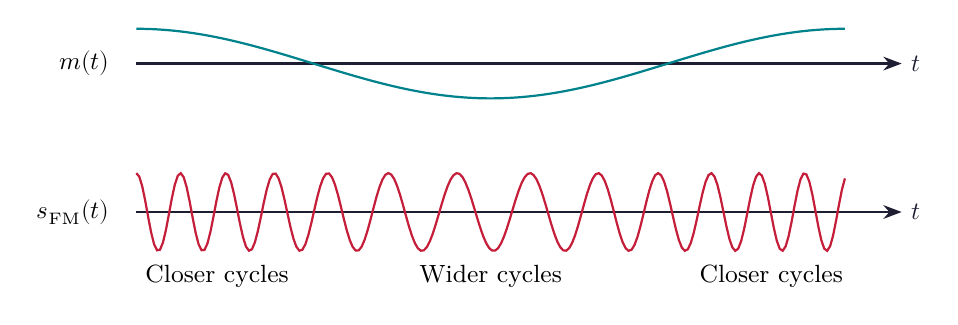
\begin{tikzpicture}[x=1.8cm,y=0.65cm,every node/.style={font=\small}]
  \draw[arrow] (0,2.9)--(5.4,2.9) node[right] {$t$};
  \draw[arrow] (0,0)--(5.4,0) node[right] {$t$};
  \draw[myteal,thick,domain=0:5,samples=100] plot (\x,{2.9+0.68*cos(72*\x)});
  \draw[myred,thick,domain=0:5,samples=240] plot (\x,{0.76*cos(930*\x+185*sin(72*\x))});
  \node[anchor=east] at (-0.12,2.9) {$m(t)$};
  \node[anchor=east] at (-0.12,0) {$s_{\rm FM}(t)$};
  \node[below] at (0.57,-0.85) {Closer cycles};
  \node[below] at (2.50,-0.85) {Wider cycles};
  \node[below] at (4.48,-0.85) {Closer cycles};
\end{tikzpicture}\par
\small Here $k_f>0$. The RF envelope remains constant at all three positions.
\end{tcolorbox}

\section{Single-Tone Spectrum and Bessel Coefficients}
\subsection{Fourier Series Representation}
The complex factor $e^{j\beta\sin\omega_mt}$ is periodic at $f_m$. Its Fourier coefficient of order $n$ is a Bessel function of the first kind:
\[
\begin{aligned}
 J_n(\beta)&=\frac{1}{2\pi}\int_{-\pi}^{\pi}
            e^{j(\beta\sin\theta-n\theta)}\,d\theta,\\
 e^{j\beta\sin\omega_mt}&=\sum_{n=-\infty}^{\infty}
            J_n(\beta)e^{jn\omega_mt}.
\end{aligned}
\]
Multiply by $A_ce^{j\omega_ct}$ and take the real part:
\[
 s_{\rm FM}(t)=A_c\sum_{n=-\infty}^{\infty}
          J_n(\beta)\cos[(\omega_c+n\omega_m)t].
\]
The signed cosine coefficient is $A_cJ_n(\beta)$. In the two-sided Fourier transform, each cosine splits into two impulses of half this weight. Positive RF lines are drawn near $f_c$ for the orders of interest. A negative coefficient denotes a $\pi$ phase reversal, not negative power. Since $\cos\omega_mt=\sin(\omega_mt+\pi/2)$, single-tone PM obeys
\[
 s_{\rm PM}(t)=A_c\sum_{n=-\infty}^{\infty}
 J_n(\beta_p)\cos[(\omega_c+n\omega_m)t+n\pi/2].
\]
The complex weights of PM at the lines $f_c+nf_m$ are $A_cJ_n(\beta_p)e^{jn\pi/2}$ in the carrier-referenced representation. The positive-frequency Fourier impulse has half this weight and its negative-frequency image has the conjugate weight. At equal indices, the FM and PM magnitude spectra coincide. Their phases differ by $n\pi/2$ at the line of order $n$.

\begin{tcolorbox}[formulabox, title={Bessel Identities and Spectrum Power}]
\[
\begin{aligned}
 J_{-n}(\beta)&=(-1)^n J_n(\beta),\\
 J_0^2(\beta)+2\sum_{n=1}^{\infty}J_n^2(\beta)&=1,\\
 P_T&=P_c\left[J_0^2(\beta)+2\sum_{n=1}^{\infty}J_n^2(\beta)\right]
      =P_c,\qquad P_c=\frac{A_c^2}{2R}.
\end{aligned}
\]
Here $P_c$ denotes unmodulated carrier power. The line remaining at $f_c$ has power $P_c J_0^2(\beta)$. It vanishes at the first root $\beta\approx2.405$ while total RF power stays constant.
\end{tcolorbox}

\begin{tcolorbox}[tikzbox, unbreakable, title={FM and PM Line Magnitudes at Index One}]
\centering
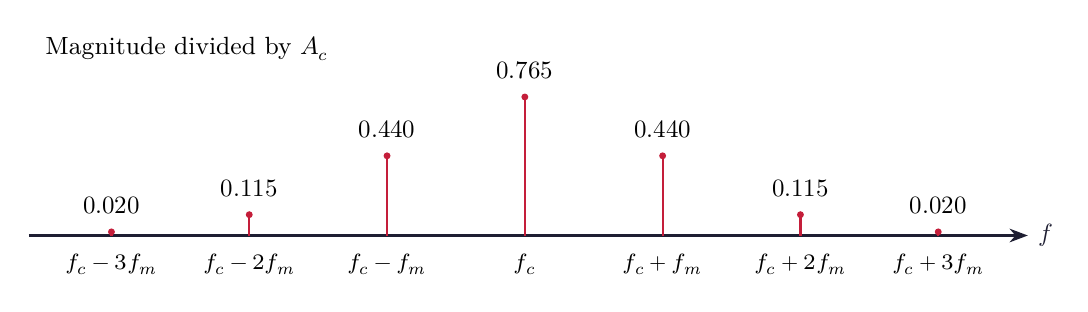
\begin{tikzpicture}[x=1.75cm,y=2.3cm,every node/.style={font=\small}]
  \draw[arrow] (-3.6,0)--(3.65,0) node[right] {$f$};
  \node[anchor=west] at (-3.55,1.03) {Magnitude divided by $A_c$};
  \foreach \n/\h/\v in {-3/0.020/0.020,-2/0.115/0.115,-1/0.440/0.440,0/0.765/0.765,1/0.440/0.440,2/0.115/0.115,3/0.020/0.020}{
    \draw[myred,thick] (\n,0)--(\n,\h);
    \fill[myred] (\n,\h) circle (1.25pt);
    \node[above=3pt] at (\n,\h) {$\v$};
  }
  \foreach \n/\ff in {-3/f_c-3f_m,-2/f_c-2f_m,-1/f_c-f_m,0/f_c,1/f_c+f_m,2/f_c+2f_m,3/f_c+3f_m}{
    \node[below=3pt] at (\n,0) {\footnotesize $\ff$};
  }
\end{tikzpicture}\par
\small For FM, the odd-order lower lines have reversed signs. For PM, apply the additional order-dependent $n\pi/2$ phase shift at the same index.
\end{tcolorbox}

\subsection{Narrowband Approximation and Phasors}
If $|\phi(t)|\ll1$ rad, expand
\[
\begin{aligned}
 s(t)&=A_c[\cos\omega_ct\cos\phi(t)-\sin\omega_ct\sin\phi(t)]\\
     &\approx A_c\cos\omega_ct-A_c\phi(t)\sin\omega_ct.
\end{aligned}
\]
For tone FM, $J_0\approx1$ and $J_{\pm1}\approx\pm\beta/2$. For tone PM, the phase factors $e^{\pm j\pi/2}$ turn the first-order coefficients into $j\beta_p/2$ on both sides. The two sideband sums in the carrier frame are
\[
\begin{aligned}
 E_{\mathrm{SB,FM}}(t)
 &= \frac{A_c\beta}{2}\bigl(e^{j\omega_mt}-e^{-j\omega_mt}\bigr)\\
 &= jA_c\beta\sin\omega_mt,\\[3pt]
 E_{\mathrm{SB,PM}}(t)
 &= \frac{jA_c\beta_p}{2}\bigl(e^{j\omega_mt}+e^{-j\omega_mt}\bigr)\\
 &= jA_c\beta_p\cos\omega_mt.
\end{aligned}
\]
In both cases the sidebands add in quadrature to the carrier. For the cosine message, the PM phase swing is in step with the message and the FM phase swing is delayed by a quarter cycle. The baseband phase and frequency deviations follow the definitions above.

\begin{tcolorbox}[tikzbox, unbreakable, title={Narrowband FM and PM Phasor Construction}]
\centering
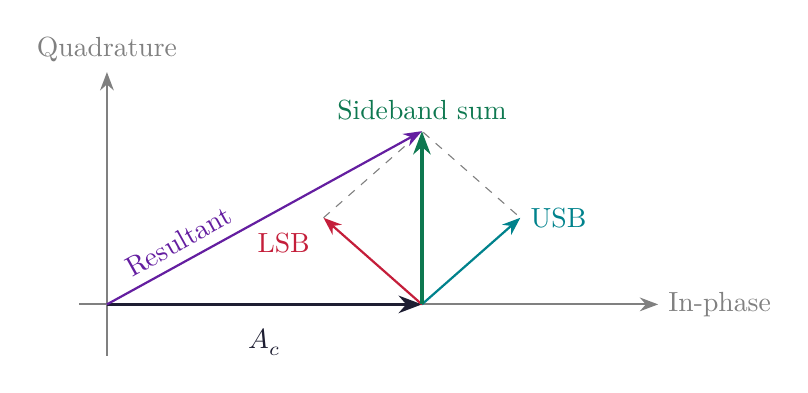
\begin{tikzpicture}
  \draw[arrow,gray] (-0.35,0)--(7,0) node[right] {In-phase};
  \draw[arrow,gray] (0,-0.65)--(0,2.95) node[above] {Quadrature};
  \draw[arrow,very thick] (0,0)--(4,0) node[midway,below=5pt] {$A_c$};
  \draw[arrow,thick,myteal] (4,0)--(5.25,1.1) node[right] {USB};
  \draw[redarrow,thick] (4,0)--(2.75,1.1);
  \node[myred,anchor=east] at (2.7,0.78) {LSB};
  \draw[dashed,gray] (2.75,1.1)--(4,2.2)--(5.25,1.1);
  \draw[arrow,mygreen,very thick] (4,0)--(4,2.2) node[above] {Sideband sum};
  \draw[arrow,mypurple,thick] (0,0)--(4,2.2);
  \node[above,rotate=29,mypurple] at (1.03,0.58) {Resultant};
\end{tikzpicture}\par
\small FM and PM share this geometry at a positive phase excursion. The sideband vectors for PM are the FM construction evaluated a quarter message period later, with the corresponding PM scale.
\end{tcolorbox}

\subsection{Wideband Angle Modulation and Carson's Rule}
When the phase deviation is not small, higher-order sidebands must be retained. The mathematical line spectrum has infinitely many orders. A useful occupied bandwidth estimate for message bandwidth $W$ and peak frequency deviation $\Delta f$ is
\[
 B_{\rm Carson}\approx 2(\Delta f+W)\quad(\mathrm{Hz}).
\]
For a tone put $W=f_m$. For PM with more than one tone, obtain $\Delta f$ from the peak of $|k_pm'(t)/(2\pi)|$. A narrowband first-order treatment gives approximately $2W$.

\begin{tcolorbox}[examplebox, title={Find Index, Line Positions and Bandwidth}]
The FM phase is $2\pi(100\times10^6)t+5\sin[2\pi(15\times10^3)t]$.
\[
\begin{aligned}
 f_c&=100\,\mathrm{MHz},& f_m&=15\,\mathrm{kHz},& \beta&=5,\\
 \Delta f&=\beta f_m=75\,\mathrm{kHz},\\
 B_{\rm Carson}&\approx 2(75+15)=180\,\mathrm{kHz}.
\end{aligned}
\]
The $n=\pm1$ lines lie at $99.985$ and $100.015\,\mathrm{MHz}$. Higher pairs are spaced by another $15\,\mathrm{kHz}$ per order. With a PM tone at the same frequency and peak phase deviation of $5$ rad, the magnitudes and Carson estimate are identical.
\end{tcolorbox}

\section{Generation of FM and PM}
\subsection{Direct FM with VCO or Reactance Modulator}
A voltage-controlled oscillator (VCO) tunes frequency through the applied voltage. Bias sets the unmodulated $f_c$. In its linear range $f_i=f_c+k_fm(t)$. A varactor changes tank capacitance. For inductance $L$ and total capacitance $C$,
\[
\begin{aligned}
 f_c &=\frac{1}{2\pi\sqrt{LC}},\\
 \Delta f&\approx-\frac{f_c}{2}\frac{\Delta C}{C}.
\end{aligned}
\]
The second line follows by differentiating $C^{-1/2}$ for a small capacitance swing. A reactance modulator makes a device draw a current approximately in quadrature with tank voltage. In one capacitive implementation $v_g\approx j\omega RC\,v$ and $i=g_m v_g$, so $i/v\approx j\omega g_mRC$. It behaves as $C_{\rm eff}\approx g_m RC$, tunable through transconductance $g_m$. A limiter stabilizes amplitude. Frequency drift and tuning nonlinearity limit direct FM unless controlled.

\subsection{Direct PM and Indirect FM (Armstrong)}
A quadrature phase modulator uses $\phi=k_pm(t)$ to control two gains, $I=\cos\phi$ and $Q=\sin\phi$. Weight the corresponding carrier branches and subtract:
\[
\begin{aligned}
 s(t)&=A_c[I\cos\omega_ct-Q\sin\omega_ct]\\
     &=A_c\cos(\omega_ct+\phi).
\end{aligned}
\]
For narrowband PM, use $I\approx1$ and $Q\approx\phi$ in the same structure. For wideband PM, use the full trigonometric gains so that $I^2+Q^2=1$ even at large phase deviation.

For indirect FM, integrate the message before the crystal-based narrowband phase modulator. The multiplier of factor $N$ multiplies $f_c$, the phase deviation and $\Delta f$ by $N$. A mixer with a fixed LO then sets the centre frequency without changing the magnitude of the deviation. This is the Armstrong route to wideband FM. The same multiplication chain can widen narrowband PM when the message integrator is bypassed.

\begin{tcolorbox}[tikzbox, unbreakable, title={Direct FM, Quadrature PM and Armstrong FM}]
\centering
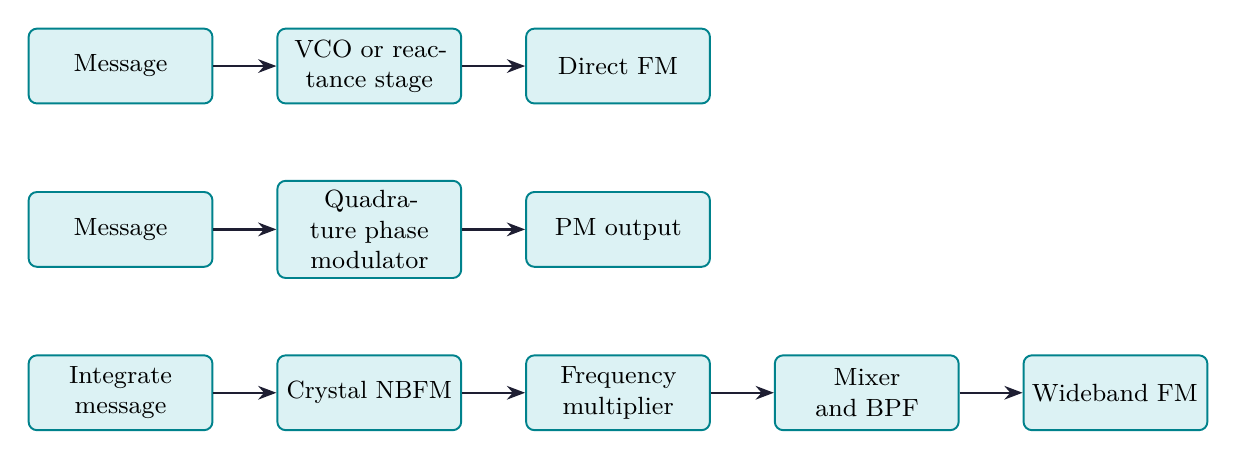
\begin{tikzpicture}[node distance=8mm,sblock/.style={block,text width=2.1cm}]
  \node[sblock] (m1) {Message};
  \node[sblock,right=of m1] (vco) {VCO or reactance stage};
  \node[sblock,right=of vco] (fm) {Direct FM};
  \draw[arrow] (m1)--(vco); \draw[arrow] (vco)--(fm);
  \node[sblock,below=11mm of m1] (m2) {Message};
  \node[sblock,right=of m2] (pm) {Quadrature phase modulator};
  \node[sblock,right=of pm] (pmo) {PM output};
  \draw[arrow] (m2)--(pm); \draw[arrow] (pm)--(pmo);
  \node[sblock,below=11mm of m2] (i) {Integrate message};
  \node[sblock,right=of i] (n) {Crystal NBFM};
  \node[sblock,right=of n] (mul) {Frequency multiplier};
  \node[sblock,right=of mul] (mix) {Mixer and BPF};
  \node[sblock,right=of mix] (out) {Wideband FM};
  \draw[arrow] (i)--(n); \draw[arrow] (n)--(mul);
  \draw[arrow] (mul)--(mix); \draw[arrow] (mix)--(out);
\end{tikzpicture}\par
\end{tcolorbox}

\pagebreak[3]
\section{Demodulation of FM and PM}
\subsection{Frequency Discriminator and PM Recovery}
A frequency discriminator produces voltage proportional to the instantaneous frequency offset within its linear range. A slope detector converts frequency changes to envelope changes using one side of a tuned response and then detects that envelope. Its output is sensitive to unwanted AM and to response curvature. A balanced discriminator subtracts the outputs of two offset responses, giving an approximately odd output near $f_c$ and improved linearity. A limiter precedes many discriminators. For gain $K_d$ in $\mathrm{V/Hz}$,
\[
 v_d(t)\approx K_d[f_i(t)-f_c].
\]
For FM, $v_d\propto m(t)$. For PM, $v_d\propto m'(t)$, so integrate and restore the reference level as required. PM may also be recovered by a phase detector comparing with a coherent carrier reference, provided the phase swing remains in the usable range or is unwrapped.

\begin{tcolorbox}[tikzbox, unbreakable, title={Balanced Frequency Discriminator}]
\centering
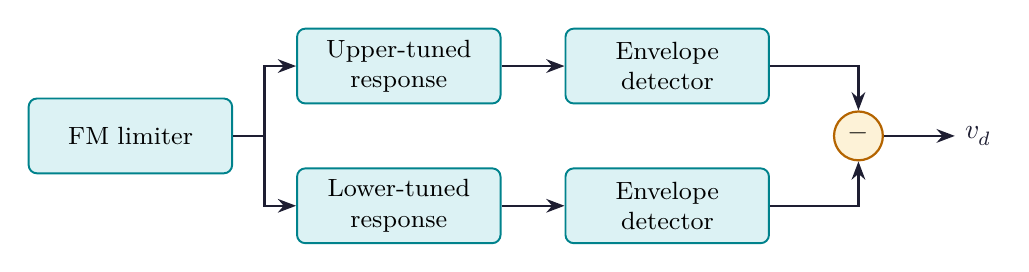
\begin{tikzpicture}[node distance=8mm,sblock/.style={block,text width=2.35cm}]
  \node[sblock] (hi) {Upper-tuned response};
  \node[sblock,below=8mm of hi] (lo) {Lower-tuned response};
  \node[sblock,right=of hi] (dh) {Envelope detector};
  \node[sblock,right=of lo] (dl) {Envelope detector};
  \coordinate (leftmid) at ($(hi.west)!0.5!(lo.west)$);
  \node[sblock,left=of leftmid] (lim) {FM limiter};
  \coordinate (rightmid) at ($(dh.east)!0.5!(dl.east)$);
  \node[sumjunc,right=of rightmid] (sub) {$-$};
  \draw[arrow] (lim.east)--++(4mm,0)|-(hi.west);
  \draw[arrow] (lim.east)--++(4mm,0)|-(lo.west);
  \draw[arrow] (hi)--(dh);
  \draw[arrow] (lo)--(dl);
  \draw[arrow] (dh.east)-|(sub.north);
  \draw[arrow] (dl.east)-|(sub.south);
  \draw[arrow] (sub.east)--++(9mm,0) node[right] {$v_d$};
\end{tikzpicture}\par
\small The two envelopes are equal at the centre frequency. Above centre the upper branch dominates, and below centre the lower branch dominates.
\end{tcolorbox}

\subsection{Phase-Locked Loop}
A PLL compares the input and VCO phases, filters the phase error, and drives the VCO to track the input. For a linearized phase detector with gain $K_p$ in $\mathrm{V/rad}$ and VCO gain $K_v$ in $\mathrm{Hz/V}$:
\[
 v_e=K_p(\theta_i-\theta_o),\qquad
 f_{\rm VCO}=f_{\rm free}+K_vv_{\rm ctrl}.
\]
When locked and tracking sufficiently fast, with $f_{\rm free}=f_c$,
\[
 v_{\rm ctrl}\approx\frac{f_i-f_c}{K_v}
                  =\frac{k_f}{K_v}m(t)\quad\text{for FM}.
\]
The control voltage yields the time derivative of the phase deviation for PM. Integration recovers that phase up to a reference constant. Capture means acquiring lock from an unlocked state. The lock range describes how far frequency may move after lock is established. Loop bandwidth trades tracking against noise rejection.

\begin{tcolorbox}[tikzbox, unbreakable, title={PLL Feedback and Demodulated Output}]
\centering
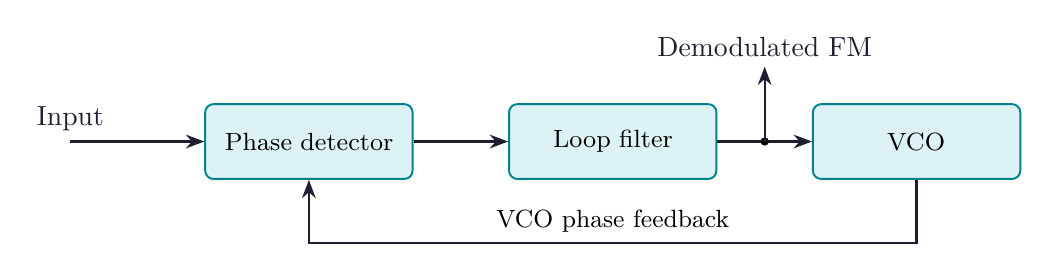
\begin{tikzpicture}[node distance=12mm]
  \node[block] (pd) {Phase detector};
  \node[block,right=of pd] (lf) {Loop filter};
  \node[block,right=of lf] (vco) {VCO};
  \draw[arrow] ([xshift=-17mm]pd.west)--(pd.west) node[pos=0,above] {Input};
  \draw[arrow] (pd)--(lf);
  \draw[arrow] (lf)--(vco);
  \coordinate (tap) at ($(lf.east)!0.5!(vco.west)$);
  \fill (tap) circle (1.5pt);
  \draw[arrow] (tap)--++(0,0.95) node[above] {Demodulated FM};
  \draw[arrow] (vco.south)--++(0,-0.8)-| (pd.south);
  \node at ($(lf.south)+(0,-0.52)$) {\small VCO phase feedback};
\end{tikzpicture}\par
\end{tcolorbox}

\begin{tcolorbox}[examplebox, title={Demodulate FM with a Locked PLL}]
Let $A_m=2\,\mathrm V$, $k_f=15\,\mathrm{kHz/V}$, $K_v=20\,\mathrm{kHz/V}$ and $f_{\rm free}=f_c$.
\[
\begin{aligned}
 \Delta f &= k_fA_m=30\,\mathrm{kHz},\\
 V_{\rm ctrl,peak} &\approx \frac{\Delta f}{K_v}=1.5\,\mathrm V.
\end{aligned}
\]
A gain of $4/3$ restores the original voltage scale while the PLL stays locked and tracks the tone.
\end{tcolorbox}

\newpage
\begin{center}
  {\large\bfseries\color{myred} Quick Revision --- Module 3}\\[3pt]
  {\small\color{mydark} Angle Modulation, Generation and Demodulation $|$ EC401}
\end{center}
\noindent{\color{myred}\rule{\linewidth}{1.2pt}}
\par\vspace{4pt}

\begin{tcolorbox}[formulabox, title={Key Formulas at a Glance}]
\renewcommand{\arraystretch}{1.35}
\noindent\begin{tabularx}{\linewidth}{B{4.4cm} Y}
Instantaneous frequency & $f_i=f_c+\phi'(t)/(2\pi)$ \\[4pt]
FM and PM phase & $\phi_{\rm FM}=2\pi k_f\int m(t)\,dt$ \newline $\phi_{\rm PM}=k_pm(t)$ \\[4pt]
Single-tone indices & $\beta=\Delta f/f_m$ for FM \quad $\beta_p=k_pA_m$ for PM \\[4pt]
Bessel spectrum & Tone lines at $f_c+nf_m$ \newline FM cosine coefficient $A_cJ_n(\beta)$ \\[4pt]
Carson estimate & $B\approx 2(\Delta f+W)$ \\[4pt]
Frequency multiplication & $f_c,\Delta f,\beta$ multiply by $N$ for tone FM \\[4pt]
FM detection & $v_d\approx K_d(f_i-f_c)$ \newline $v_{\rm ctrl}\approx(f_i-f_c)/K_v$ while tracking in lock \\[4pt]
\end{tabularx}\par
\end{tcolorbox}

\begin{tcolorbox}[defbox, title={One-Line Definitions}]
\begin{itemize}[leftmargin=*, itemsep=3pt, topsep=0pt]
  \item \textbf{Deviation.} Peak magnitude of $f_i-f_c$ in hertz.
  \item \textbf{Bessel coefficient.} Fourier-series coefficient of the single-tone angle-modulation factor.
  \item \textbf{Discriminator.} Converts instantaneous frequency offset to voltage.
  \item \textbf{PLL.} Feedback loop that tracks the input carrier phase.
\end{itemize}
\end{tcolorbox}

\begin{tcolorbox}[exambox, title={Frequently Asked / Viva Questions}]
\begin{enumerate}[topsep=0pt, label=\textbf{Q\arabic*.}, itemsep=5pt]
  \item \Q{Which carrier property stays constant?}
    Peak amplitude stays constant in ideal FM and PM.
  \item \Q{How can a PM circuit generate FM?}
    Integrate the message before applying it to the phase modulator.
  \item \Q{What happens to the PM frequency deviation as tone frequency increases?}
    It increases as $\Delta f_{\rm PM}=k_pA_mf_m$ for fixed amplitude.
  \item \Q{Why can the FM carrier line disappear?}
    $J_0(\beta)$ can be zero. The power is redistributed among sidebands.
  \item \Q{What does a negative Bessel coefficient mean?}
    A $\pi$ phase reversal of that cosine component. Its contribution to power stays positive.
  \item \Q{Why is the NBFM sideband sum in quadrature?}
    The opposite signed first-order coefficients cancel the horizontal projections and add the vertical ones.
  \item \Q{Why use a multiplier in Armstrong FM?}
    It increases the deviation of a stable narrowband source. A mixer then sets the desired channel centre.
  \item \Q{How does a reactance modulator tune FM?}
    A control voltage varies the effective reactive admittance of the oscillator tank.
  \item \Q{How does a discriminator recover PM?}
    Its output is proportional to the message derivative. Integrate to recover the original message up to a reference constant.
  \item \Q{What makes the PLL control voltage useful for FM?}
    While locked and tracking, it supplies the VCO frequency correction and is proportional to $m(t)$.
\end{enumerate}
\end{tcolorbox}

\begin{tcolorbox}[tikzbox, unbreakable, title={Summary Comparison}]
\begingroup
\setlength{\tabcolsep}{5pt}
\setlength{\extrarowheight}{3pt}
\renewcommand{\arraystretch}{1.45}
\noindent\begin{tabularx}{\linewidth}{|B{3.35cm}|Y|Y|}
\hline
\multicolumn{1}{|c|}{\textbf{Feature}} & \multicolumn{1}{c|}{\textbf{Frequency modulation}} & \multicolumn{1}{c|}{\textbf{Phase modulation}} \\
\hline
Directly controlled & $f_i-f_c=k_fm(t)$ & $\phi=k_pm(t)$ \\
\hline
Tone frequency deviation & $k_fA_m$ & $k_pA_m f_m$ \\
\hline
Before alternate modulator & Integrate before PM. & Differentiate before FM. \\
\hline
After discriminator & Scale directly. & Integrate and scale. \\
\hline
\end{tabularx}\par
\endgroup
\end{tcolorbox}

\end{document}
